\documentclass[11pt]{article}

\usepackage[T1]{fontenc}
\usepackage{bookmark}
\usepackage{amsmath, amsthm, amssymb, amsfonts, mathrsfs}
\usepackage{thmtools}
\usepackage{graphicx}
\usepackage{setspace}
\usepackage{geometry}
\usepackage{float}
\usepackage{hyperref}
\usepackage{framed}
\usepackage[dvipsnames,svgnames]{xcolor}
\usepackage{tikz-cd}
\usepackage{circuitikz}
\usepackage[most]{tcolorbox}
\usepackage{enumitem}
\usepackage[center]{titlesec}
% \usepackage{mypackage} % 你的常用符号包，按需启用
\usepackage{fontawesome5}
\usetikzlibrary{positioning}

\usepackage{pgfplots}
\pgfplotsset{compat=newest}

\usepackage[backend=biber,style=alphabetic,sorting=none]{biblatex}
\addbibresource{reference.bib} % 按需启用

\tcbuselibrary{theorems}
\tcbuselibrary{breakable}

% ---------- 颜色定义 ----------
\colorlet{LightGray}{White!90!Periwinkle}
\colorlet{LightOrange}{Orange!10}
\colorlet{LightGreen}{Green!10}
\colorlet{Lightblue}{Blue!10}
\colorlet{Lightpurple}{Purple!10}
\colorlet{LightRed}{Red!10}
\colorlet{LightYellow}{Yellow!10}
\colorlet{LightCyan}{Cyan!10}
\colorlet{LightAquamarine}{Aquamarine!10}
\colorlet{LightCadetBlue}{CadetBlue!10}

\newcommand{\HRule}[1]{\rule{\linewidth}{#1}}

% ---------- 定理环境（英文） ----------
\declaretheoremstyle[
  name = Theorem,
  postheadspace={\newline},
]{thmsty}

\declaretheorem[
  style=thmsty,
  numberwithin=section,
  refname={Theorem},
]{theorem}
\tcolorboxenvironment{theorem}{
  colback=LightGray,
  breakable,
  before upper app={\setlength{\parindent}{2em}}
}

\declaretheoremstyle[name=Definition,]{thmsty}
\declaretheorem[style=thmsty,sibling=theorem,refname={Definition}]{definition}
\tcolorboxenvironment{definition}{colback=LightCyan,breakable,before upper app={\setlength{\parindent}{2em}}}

\declaretheoremstyle[name=Remark,]{thmsty}
\declaretheorem[style=thmsty,sibling=theorem,refname={Remark}]{remark}
\tcolorboxenvironment{remark}{colback=LightRed,breakable,before upper app={\setlength{\parindent}{2em}}}

\declaretheoremstyle[name=Lemma,]{thmsty}
\declaretheorem[style=thmsty,sibling=theorem,refname={Lemma}]{lemma}
\tcolorboxenvironment{lemma}{colback=Lightblue,breakable,before upper app={\setlength{\parindent}{2em}}}

\declaretheoremstyle[name=Corollary,]{thmsty}
\declaretheorem[style=thmsty,sibling=theorem,refname={Corollary}]{corollary}
\tcolorboxenvironment{corollary}{colback=Lightpurple,breakable,before upper app={\setlength{\parindent}{2em}}}

\declaretheoremstyle[name=Proposition,]{prosty}
\declaretheorem[style=prosty,sibling=theorem,refname={Proposition}]{proposition}
\tcolorboxenvironment{proposition}{colback=LightOrange,breakable,before upper app={\setlength{\parindent}{2em}}}

\declaretheoremstyle[name=Example,]{prosty}
\declaretheorem[style=prosty,sibling=theorem,refname={Example}]{example}
\tcolorboxenvironment{example}{colback=LightGreen,breakable,before upper app={\setlength{\parindent}{2em}}}

\declaretheoremstyle[name=Exercise,]{prosty}
\declaretheorem[style=prosty,numberwithin=section]{exercise}
\tcolorboxenvironment{exercise}{colback=LightAquamarine,breakable,before upper app={\setlength{\parindent}{2em}}}

\declaretheoremstyle[name=Answer,]{prosty}
\declaretheorem[style=prosty,numberwithin=section]{answer}
\tcolorboxenvironment{answer}{colback=LightCadetBlue,breakable,before upper app={\setlength{\parindent}{2em}}}

% ---------- 罗马数字 ----------
\makeatletter
\newcommand{\rmnum}[1]{\romannumeral #1}
\newcommand{\Rmnum}[1]{\expandafter\@slowromancap\romannumeral #1@}
\makeatother

% ---------- 标题格式 ----------
% article 没有 \chapter，因此删除 \titleformat{\chapter}
\titleformat{\section}{\raggedright\Large\bfseries}{\,\thesection\,}{1em}{}
\titleformat{\subsection}{\raggedright\large\bfseries}{\,\thesubsection\,}{1em}{}

\setstretch{1.2}
\geometry{
    textheight=9in,
    textwidth=5.5in,
    top=1in,
    headheight=12pt,
    headsep=25pt,
    footskip=30pt
}


% ------------------------------------------------------------------------------

\newcommand{\im}{\operatorname{im}}
\newcommand{\id}{\operatorname{id}}
\newcommand{\coker}{\operatorname{coker}}
\newcommand{\PSh}{\mathsf{PSh}}
\newcommand{\Sh}{\mathsf{Sh}}
\newcommand{\sh}{\operatorname{sh}}
\newcommand{\Hom}{\operatorname{Hom}}

% ---------- 文档信息 ----------
\title{\textbf{Seminar On Algebraic Geometry\\ Lecture Notes 2}}
\title{%
  \vspace*{-2cm}
  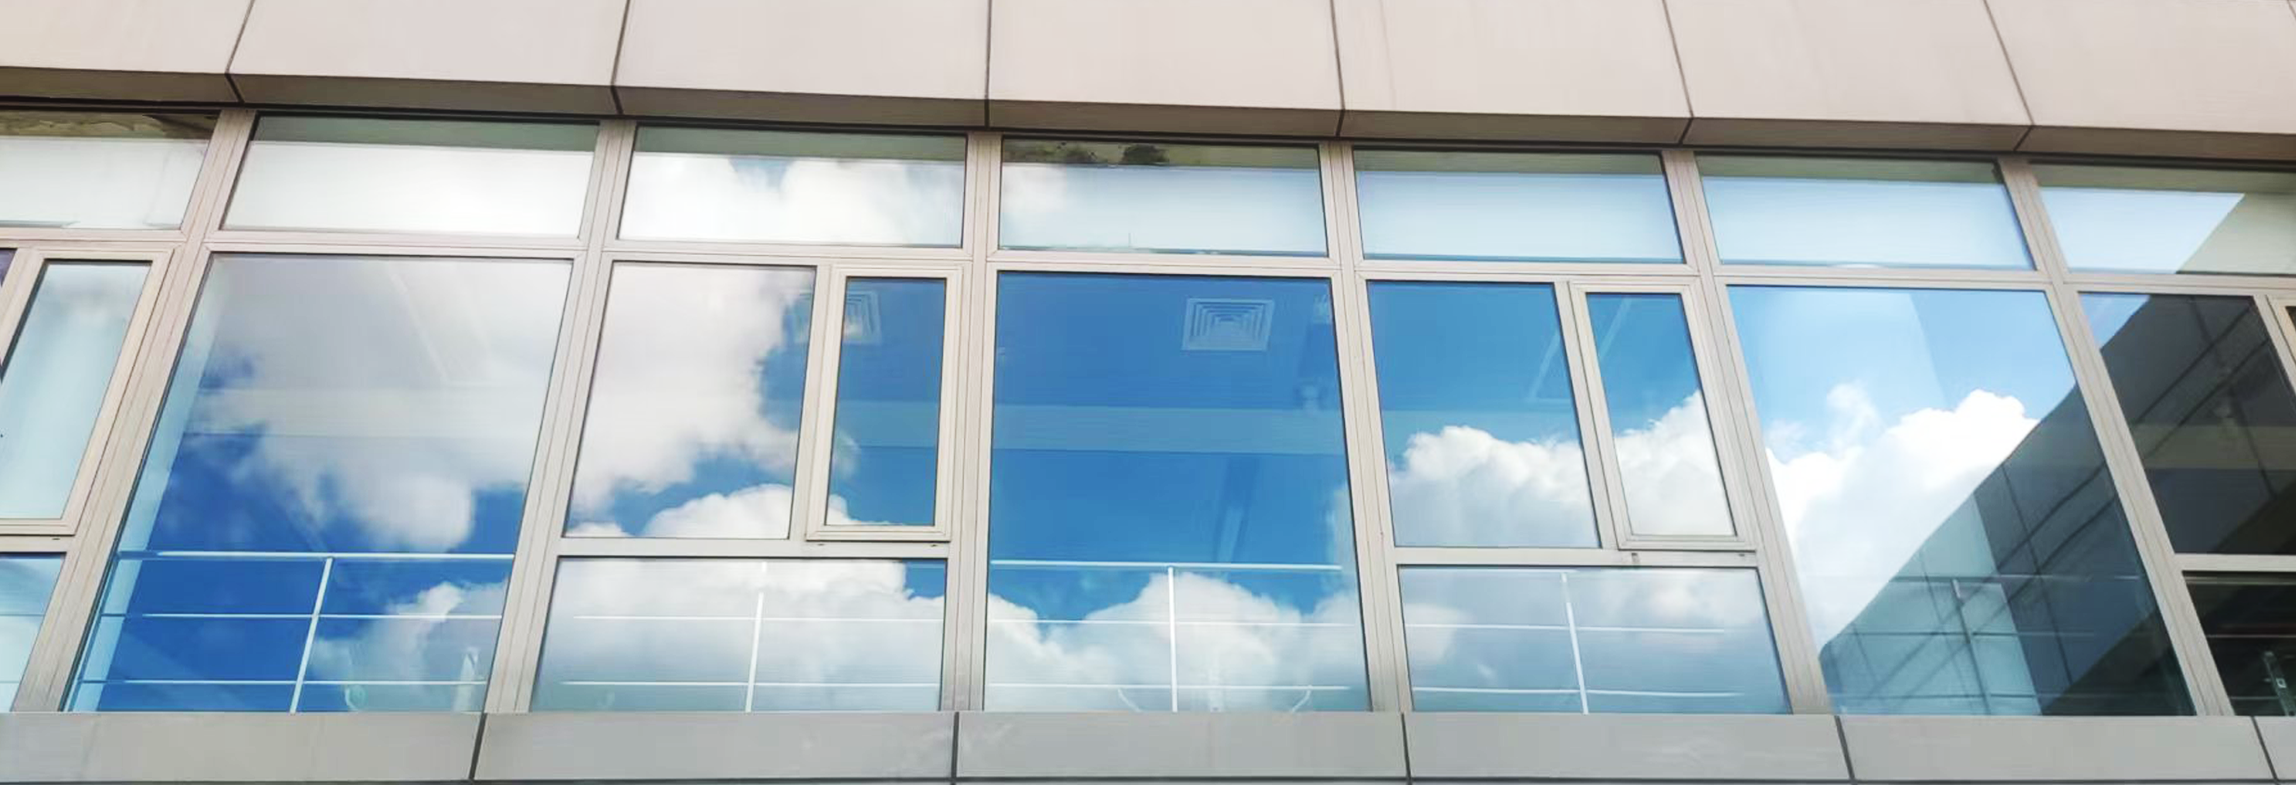
\includegraphics[width=\textwidth]{SKy.png}\\[1.2cm]
  \textbf{Seminar On Algebraic Geometry\\ Lecture Notes 2 (Incomplete version)}%
}
\author{Zihang Zhang}
\date{October 19, 2026}

\begin{document}


\maketitle
\thispagestyle{empty}

\tableofcontents
\newpage

In this lecture, we will discuss sheaves of abelian groups (moreover, sheaves of modules) 
by viewing $ \Sh $ as an abelian category. 

\section{Abelian Category Of Sheaves}

Let $ X $ be a topological space. 

\begin{definition}
  Let $\mathscr{F}'$ be a subsheaf of a sheaf $\mathscr{F}$, 
  i.e. there is an injective morphism $ i:\mathscr{F}' \to \mathscr{F} $ 
  (we can view $ \mathscr{F}'(U) $ as a subsheaf of $ \mathscr{F}(U) $ for each open subset $ U $). 
  We define the quotient sheaf $\mathscr{F} / \mathscr{F}'$ to be the sheafification 
  of the presheaf $U \mapsto \mathscr{F}(U) / \mathscr{F}'(U)$. 
  For any $ P \in X $, we have $ (\mathscr{F} / \mathscr{F}')_{P} = \mathscr{F}_{P} / \mathscr{F}'_{P} $. 
\end{definition}

\begin{corollary}
  \cite[Exercise II.1.7]{hartsAG}
  Let $\varphi:\mathscr{F} \to \mathscr{G}$ be a morphism of sheaves. 
  Then $\im\varphi \cong \mathscr{F} / \ker \varphi$, and 
  $\mathrm{coker}\,\varphi \cong \mathscr{G} / \mathrm{im}\,\varphi$. 
\end{corollary}

\begin{proposition}[Direct sum]
  \cite[Exercise II.1.9]{hartsAG}
\end{proposition}

\begin{proposition}[Direct limit]
  \cite[Exercise II.1.10, 1.11]{hartsAG}
\end{proposition}

\begin{proposition}[Inverse limit]
  \cite[Exercise II.1.12]{hartsAG}
\end{proposition}



\section{Operations on Sheaves}

\subsection{Global Section Functor}

Recall that we sometimes write $ \Gamma(U,\mathscr{F}):= \mathscr{F}(U)$, 
for any open subset $ U \subseteq X $ and any sheaf $ \mathscr{F} $ on $ X $. 

\begin{proposition}
  \label{prop: left-exactness of Gamma}
    \cite[Ex 1.8]{hartsAG} 
    Suppose $U \subseteq X$ is an open subset, 
    and $0 \to \mathscr{F} \to \mathscr{G} \to \mathscr{H}$ is an exact sequence 
    of sheaves of abelian groups. 
    Then $$0 \to \Gamma(U,\mathscr{F}) \to \Gamma(U,\mathscr{G}) \to \Gamma(U,\mathscr{H})$$
    is exact. I.e., $ \Gamma(U,-) $  is a left exact functor $\mathrm{Sh}(X) \to \mathrm{Ab}$. 
\end{proposition}

\begin{proof}
  We can easily check this on the level of stalks, 
  since for any morphism $ \varphi: \mathscr{F} \to \mathscr{G} $ of sheaves, 
  and for any $ P \in U $, we have $ \ker \varphi_{P} = (\ker \varphi)_{P} $ and 
  $ \im \varphi_{P} = (\im \varphi)_{P} $.  
\end{proof}

However, $ \Gamma(U,-) $ is not exact in general, especially in algebraic geometry:
a surjective morphism of sheaves need not induce a surjection on sections. 
The following two examples illustrate that differential topology is ``soft,'' 
whereas the Zariski topology is ``hard.'' 

\begin{lemma}
  \label{lemma: partition of units}
  Let $ M $ be a smooth (paracompact) manifold and let $ \{U_{i}\}_{i \in I} $ be an open cover of $ M $. 
  Then there exists a locally finite partition of unity subordinate to $ \{U_{i}\} $: 
  a family $ \{\rho_{i}\}_{i \in I} $ of smooth functions $ \rho_{i} \in C^{\infty}(M) $ such that 
  $ 0 \le \rho_{i} \le 1 $, $ \operatorname{supp}\rho_{i} \subseteq U_{i} $ is compact, 
  the family $ \{\operatorname{supp}\rho_{i}\}_{i \in I} $ is locally finite, and 
  $ \sum_{i \in I} \rho_{i} = 1 $ on $ M $ (the sum is locally finite, hence well defined).
\end{lemma}

\begin{example}
  Let $ M $ be a smooth manifold, $ \mathscr{C}^{\infty}_{M} $ the sheaf of smooth functions on $ M $, 
  and $ \mathscr{C}^{\infty}_{M,c} $ the presheaf of compactly supported smooth functions. 
  The inclusion $ \mathscr{C}^{\infty}_{M,c} \hookrightarrow \mathscr{C}^{\infty}_{M} $ induces an isomorphism 
  $$ (\mathscr{C}^{\infty}_{M,c})^{\sh} \xrightarrow{\sim} \mathscr{C}^{\infty}_{M} $$
  on sheafification. Indeed, for each $ f \in C^{\infty}(M) $ and each point, choose a locally finite open cover 
  $ \{U_{i}\}_{i \in I} $ of $ M $ by relatively compact open subsets and a partition of unity 
  $ \{\rho_{i}\}_{i \in I} $ subordinate to it. Then each $ f_{i} := \rho_{i} f $ is compactly supported 
  and only finitely many $ f_{i} $ are nonzero near each point, so $ f = \sum_{i} f_{i} $ 
  with $ \sum_{i} f_{i} \in \Gamma(M,\mathscr{C}^{\infty}_{M,c}) $. 
  Thus every smooth function is locally a sum of compactly supported smooth functions, 
  and the sheafification of $ \mathscr{C}^{\infty}_{M,c} $ is $ \mathscr{C}^{\infty}_{M} $.
\end{example}

\begin{proposition}
  Let $ M $ be a smooth manifold and $ \mathscr{O}_{M} := \mathscr{C}^{\infty}_{M} $ the sheaf of smooth functions. 
  Then the global section functor 
  $$ \Gamma(M,-) : \mathscr{O}_{M}\text{-}\mathsf{Mod} \longrightarrow \mathsf{Ab} $$
  is exact.
\end{proposition}

\begin{proof}
  Since $ \Gamma(M,-) $ is left exact, it suffices to show that every surjective morphism 
  $ \varphi : \mathscr{F} \to \mathscr{G} $ of $ \mathscr{O}_{M} $-modules induces a surjection on global sections. 
  Let $ g \in \Gamma(M,\mathscr{G}) $. As $ \varphi $ is an epimorphism of sheaves, there exist an open cover 
  $ \{U_{i}\}_{i \in I} $ of $ M $ and local lifts $ f_{i} \in \mathscr{F}(U_{i}) $ with 
  $ \varphi(f_{i}) = g|_{U_{i}} $. Choose a partition of unity $ \{\rho_{i}\}_{i \in I} $ subordinate to 
  $ \{U_{i}\}_{i \in I} $. Since $ \mathscr{F} $ is an $ \mathscr{O}_{M} $-module, the section 
  $ \rho_{i} f_{i} \in \mathscr{F}(U_{i}) $ vanishes near the boundary of $ U_{i} $, hence extends by zero 
  to a global section $ \widetilde{\rho_{i} f_{i}} \in \Gamma(M,\mathscr{F}) $. 
  By local finiteness the sum $ f := \sum_{i \in I} \widetilde{\rho_{i} f_{i}} $ is a well-defined global section of $ \mathscr{F} $, and
  $$ \varphi(f) = \sum_{i \in I} \rho_{i}\,\varphi(f_{i}) = \sum_{i \in I} \rho_{i}\, g|_{U_{i}} = g . $$
  Hence $ \varphi $ is surjective on global sections, and $ \Gamma(M,-) $ is exact.
\end{proof}

\begin{example}
  \cite[Example 2.4.10]{vakilTheRisingSea}
  Let $X=\mathbb{C}$ with the classical topology, 
  and define $\mathscr{O}_{X}$ to be the sheaf of holomorphic functions, 
  and $\mathscr{O}_{X}^{*}$ to be the sheaf of invertible holomorphic functions. 
  Then we have an exact sequence 
  $$0 \xrightarrow{\quad \quad} \underline{\mathbb{Z}} 
  \xrightarrow{\quad \times 2 \pi i \quad} \mathscr{O}_{X} 
  \xrightarrow{\quad \mathrm{exp} \quad} \mathscr{O}_{X}^{*} 
  \xrightarrow{\quad  \quad}1,$$
  where $\underline{\mathbb{Z}}$ is the constant sheaf associated to $\mathbb{Z}$. 

  Indeed, we can check this on stalks. Without loss of generality, consider $ P=0 $/ 
  Then $ \underline{\mathbb{Z}}_{0} = \mathbb{Z} $, 
  and $ \mathscr{O}_{X,0} $ is the ring of convergent Taylor series at origin, 
  and $ \mathscr{O}_{X,0}^{*} $ is the ring of functions in $  \mathscr{O}_{X,0} $ 
  which doesn't vanish at $ 0 $. The image of $ \times 2 \pi i $ on stalks 
  is $ 2 \pi i \mathbb{Z}$ as constant functions, and the kernel of $ \exp $ is just 
  $ 2 \pi i \mathbb{Z} $ by Euler's equation. 
  To show that the expotential map is surjective on stalks, we only need to notice that 
  for any holomorphic function $ f \in \mathscr{O}_{X,0}^{*} $, 
  there is an open neighborhood $ U $ of the origin such that $ f $ has no roots in $ U $. 
  Thus, $ \ln f $ is a holomorphic function in $ U $, which gives the preimage of $ f $ 
  in $ \mathscr{O}_{X,0} $. 

  Let $ U = \mathbb{C} \setminus \{0\} $ be the punctured complex plane. 
  Suppose that there is some $ f \in \mathscr{O}_{X}(U) $, such that 
  $ \exp f = \id_{U} \in \mathscr{O}_{X}^{*}(U)$, i.e., $ \exp(f(z))=z $ on $ U $. 
  Then $ f'(z)z = f'(z) e^{f(z)} = 1 $, for $ z \in U $, and we have $ f'(z) = 1/z $. 
  Now we calculate the integral at 
  $\gamma:|z|=1$: 
  $$\oint_{\gamma} f'(z) \,\mathrm{d}z = \oint_{\gamma} \frac{1}{z} \,
  \mathrm{d}z =2 \pi i  \neq 0.$$
  However, by Cauchy's Integral Theorem, since $\gamma$ is a closed curve 
  containing in $U$, a holomorphic open domain of $f'(z)$, 
  the integral must be zero. 
  Therefore, such $f$ does not exist, and $\exp(U)$ is not surjective. 
\end{example}

\subsection{Hom Sheaf}

\begin{proposition}
  \cite[Exercise II.1.15]{hartsAG}
  Let $\mathscr{F},\mathscr{G}$ be sheaves of abelian groups on $X$. 
  For any open set $U \subseteq X$, the set 
  $\mathscr{H}{om}\,(\mathscr{F}\mid_{U},\mathscr{G}\mid_{U})$ 
  is an abelian group, and $\mathscr{H}{om}(\mathscr{F},\mathscr{G})$ 
  is a sheaf of abelian groups on $X$, 
  by $U \mapsto \mathrm{Hom}\,(\mathscr{F}\mid_{U},\mathscr{G}\mid_{U})$. 
  It is called the \emph{sheaf of local morphisms} 
  of $\mathscr{F}$ into $\mathscr{G}$, 
  "sheaf hom" for short, and is denoted $\mathrm{Hom}\,(\mathscr{F},\mathscr{G})$. 
\end{proposition}

\begin{proof}
  For each open $U\subseteq X$, the set $\mathrm{Hom}(\mathscr{F}\mid_U,\mathscr{G}\mid_U)$ becomes an abelian group under pointwise addition: for morphisms $\varphi,\psi$ and any open $V\subseteq U$, $s\in\mathscr{F}(V)$, put
  \[
    (\varphi+\psi)(V)(s)=\varphi(V)(s)+\psi(V)(s),
  \]
  and define $(-\varphi)(V)(s)=-\varphi(V)(s)$, the zero morphism sending every section to $0$. The group axioms are inherited from the abelian groups $\mathscr{G}(V)$, so $U\mapsto\mathrm{Hom}(\mathscr{F}\mid_U,\mathscr{G}\mid_U)$ is a presheaf of abelian groups.

  It remains to check the sheaf axioms. Let $U\subseteq X$ be open and $\{U_i\}_{i\in I}$ an open cover of $U$.
  \emph{Identity:} if $\varphi\in\mathrm{Hom}(\mathscr{F}\mid_U,\mathscr{G}\mid_U)$ satisfies $\varphi|_{U_i}=0$ for all $i$, then for every open $V\subseteq U$ and $s\in\mathscr{F}(V)$ the sections $\varphi(V)(s)|_{V\cap U_i}=0$ for all $i$; since $\mathscr{G}$ is a sheaf and $\{V\cap U_i\}_{i\in I}$ covers $V$, we get $\varphi(V)(s)=0$, hence $\varphi=0$.
  \emph{Gluing:} suppose $\varphi_i\in\mathrm{Hom}(\mathscr{F}\mid_{U_i},\mathscr{G}\mid_{U_i})$ satisfy $\varphi_i|_{U_i\cap U_j}=\varphi_j|_{U_i\cap U_j}$ for all $i,j$. For open $V\subseteq U$ and $s\in\mathscr{F}(V)$, the sections $\varphi_i(V\cap U_i)(s|_{V\cap U_i})\in\mathscr{G}(V\cap U_i)$ agree on the overlaps $V\cap U_i\cap U_j$; by the sheaf property of $\mathscr{G}$ they glue to a unique section $\varphi(V)(s)\in\mathscr{G}(V)$. The assignments $V\mapsto\varphi(V)$ define a morphism of sheaves $\mathscr{F}\mid_U\to\mathscr{G}\mid_U$, and $\varphi|_{U_i}=\varphi_i$ by construction. Hence the presheaf is a sheaf of abelian groups.
\end{proof}

\begin{proposition}
  \cite[Exercise 2.6.I]{vakilTheRisingSea}
  Suppose $\mathscr{F}$ is a sheaf of abelian groups on a topological space $X$. 
  Then $\mathscr{H}{om}\,(\mathscr{F},\cdot)$ is a left-exact functor 
  $\mathrm{Sh}(X) \to \mathrm{Sh}(X)$, a
  nd $\mathscr{H}{om}\,(\cdot,\mathscr{F})$ is a left-exact contravariant 
  functor $\mathrm{Sh}(X) \to \mathrm{Sh}(X)$, as we define above. 
\end{proposition}

\begin{proof}
  Since the Hom sheaf is defined on sections by
  $\mathscr{H}{om}(\mathscr{F},\mathscr{G})(U)=\mathrm{Hom}(\mathscr{F}\mid_U,\mathscr{G}\mid_U)$,
  and exactness of a sequence of sheaves is checked on every open set (restriction to an open subset preserves exactness), it suffices to prove the corresponding exactness of $\mathrm{Hom}$ in $\mathrm{Sh}(U)$ for each open $U$.

  Let $0\to\mathscr{G}'\xrightarrow{\alpha}\mathscr{G}\xrightarrow{\beta}\mathscr{G}''$ be exact. We show that
  \[
    0\to\mathrm{Hom}(\mathscr{F},\mathscr{G}')\xrightarrow{\alpha_*}\mathrm{Hom}(\mathscr{F},\mathscr{G})\xrightarrow{\beta_*}\mathrm{Hom}(\mathscr{F},\mathscr{G}'')
  \]
  is exact. If $\alpha\circ\varphi=0$, then $\varphi=0$ since $\alpha$ is injective; hence $\alpha_*$ is injective. As $\beta\circ\alpha=0$, we have $\beta_*\circ\alpha_*=0$. Conversely, if $\beta\circ\varphi=0$, then $\varphi$ factors through $\ker\beta=\operatorname{im}\alpha\cong\mathscr{G}'$ (using that $\alpha$ is injective), so $\varphi=\alpha\circ\psi$ for a unique $\psi\in\mathrm{Hom}(\mathscr{F},\mathscr{G}')$. Thus $\ker\beta_*=\operatorname{im}\alpha_*$, proving left-exactness of $\mathscr{H}{om}(\mathscr{F},\cdot)$.
\end{proof}


\section{Pushforward \& Inverse Image}

\begin{definition}
  Let $f: X \to Y$ be a continuous map of topological spaces.
  \begin{itemize}
    \item For any sheaf $ \mathscr{F} $ on $ X $, we define the \emph{direct image (pushforward)} 
    sheaf $ f_{*}\mathscr{F} $ on $ Y $ by $$ f_{*}\mathscr{F}(V):=\mathscr{F}(f^{-1}V),$$ 
    for any open set $ V \subseteq Y $. 
    \item For any sheaf $ \mathscr{G} $ on $ Y $, we define a  
    presheaf 
    $ f^{+}\mathscr{G} $ on $ X $ by $$ f^{+}\mathscr{G}(U)=
    \varinjlim_{V \supseteq f(U)} \mathscr{G}(V),$$ 
    for any open set $ U \subseteq X $. And we define \emph{inverse image} 
    sheaf $ f^{-1}\mathscr{G} $ to be the sheafification of $ f^{+}\mathscr{G} $ given above.  
  \end{itemize}

  Then $f_{*}:\mathrm{Sh}(X) \to \mathrm{Sh}(Y)$ and $f^{-1}:\mathrm{Sh}(Y) \to \mathrm{Sh}(X)$ 
  are two functors between sheaves on different topological spaces. 
\end{definition}

It's easy to verify that the pushforward $ f_{*}\mathscr{F} $ is still a sheaf, 
since for any open subset $ V \subseteq Y $, $ f^{-1}V $ is an open subset of $ X $. 
However, let $ U \subseteq X $ be an open subset, it's not in general $ f(V) $ is still open. 
Therefore, we take an approximation by the larger open sets $ V \supseteq f(U) $. 
More precisely, since the inclusion determines a reversed restriction map, 
we define the inverse image to be the limit of such $ \mathscr{G}(V) $, 
with arrows $ \mathscr{G}(V) \to f^{-1}\mathscr{G}(U) $. 

If $ x \in X $ is a point, and $ i: \{x\} \hookrightarrow X $ is the inclusion map, 
then the stalk can be viewed as $ \mathscr{F}_{x}= i^{-1}\mathscr{F} $ for every presheaf $ \mathscr{F} $ 
on $ X $. 

\begin{lemma}
  \label{lemma: stalks of image}
  \cite[Exercise 2.2.I, 2.7.C]{vakilTheRisingSea}
  Suppose $ f:X \to Y $ is a continuous map, and $ \mathscr{F} $ is a sheaf on $ X $, 
  $ \mathscr{G} $ is a sheaf on $ Y $. 
  If $ f(p)=q $, then we have 
  $$ (f_{*}\mathscr{F})_{q} \cong \mathscr{F}_{p},\,\,\text{and}\,\, 
  \mathscr{G}_{q} \cong (f^{-1} \mathscr{G})_{p}.$$   
\end{lemma}

\begin{proof}
  We prove this statement by the definition of colimit. 
  On the one hand, for each open neighborhood $ U $ of $ q $, $ f^{-1}U $ is an open neighborhood 
  of $ p $, thus there is a morphism 
  $ \mathscr{F}_{p} \to  \varinjlim_{q \in U}\mathscr{F}(f^{-1}U) = (f_{*}\mathscr{F})_{q} $; 
  on the other hand, for each open neighborhood $ V $ of $ p $, $ V \subseteq f^{-1}f(V) $ 
  and $ q \in f(V) $, which shows that $ \mathscr{F}_{p} \cong (f_{*}\mathscr{F})_{q} $, 
  since the limit is given by the inclusions of open subsets. 
  
  The analogue of inverse image is given by the equation 
  $$ (f^{-1}\mathscr{G})_{p} = (f^{+}\mathscr{G})_{p} =  \varinjlim_{p \in U} 
  \varinjlim_{f(U) \subseteq V}\mathscr{G}(V)
  = \varinjlim_{q \in V}\mathscr{G}(V), $$ 
  where the last equation is because for each open neighborhood $ V $ of $ q $, 
  $q \in f^{-1}(V) $ and $ ff^{-1}(V) \subseteq V $.  
\end{proof}

\begin{proposition}
  \label{prop: image adjoint}
  \cite[Exercise II.1.18]{hartsAG}
  Let $f: X \to Y$ be a continuous map of topological space. 
  Then $f^{-1}:\mathrm{Sh}(Y) \to \mathrm{Sh}(X)$ is left-adjoint 
  to $f_{*}:\mathrm{Sh}(X)\to \mathrm{Sh}(Y)$. 
  Precisely, there is a natural isomorphism 
  $$\tau_{\mathscr{F}\mathscr{G}}:
  \mathrm{Hom}_{X}\,(f^{-1}\mathscr{G},\mathscr{F})\to \mathrm{Hom}_{Y}
  \,(\mathscr{G},f_{*}\mathscr{F})$$ 
  for any sheaf $\mathscr{F}\in \mathrm{Sh}(X)$ and $\mathscr{G}\in \mathrm{Sh}(Y)$. 
\end{proposition}

\begin{proof}
  We prove the adjointness by giving the unit and counit. 
  Notice that for open subset $ V \subseteq Y $, there is a natural morphism 
  $$\eta_{\mathscr{G}}(V): \mathscr{G}(V) \to f_{*}f^{+}\mathscr{G}(V)=\varinjlim_{V' \supseteq f(f^{-1}V)} \mathscr{G}(V')
  = \varinjlim_{V' \supseteq V \cap f(X)} \mathscr{G}(V'), $$
  since $ V \supseteq V \cap f(X)$. On the other side, for open subset $ U \subseteq X $, there is also a natural morphism 
  $$ \varepsilon_{\mathscr{F}}(U): f^{+}f_{*}\mathscr{F}(U)=
  \varinjlim_{U' \supseteq f(U)}\mathscr{F}(f^{-1}U') \to \mathscr{F}(U), $$
  since $ U $ is contained in each $ f^{-1}U' $.  
\end{proof}




\begin{definition}
  If $Z$ is a subset of $X$, regarded as a topological subspace with the induced topology
  , if $i: Z \to  X$ is the inclusion map, and if $\mathscr{F}$ is a sheaf on $X$, 
  then we call $i^{-1}\mathscr{F}$ the \emph{restriction} of $\mathscr{F}$ to $Z$, 
  and we often denote it by $\mathscr{F}\mid_{Z}$. 
  If $ U $ is an open subset of $ X $, then $ \mathscr{F}\mid_{U} $ is 
  naturally defined by $ \mathscr{F}\mid_{U}(V) = \mathscr{F}(V) $ for any open subset 
  $ V \subseteq U $. 
\end{definition}

\begin{corollary}
  Let $ Z $ be a subset of $ X $, $ \mathscr{F} $ be a sheaf on $ X $. 
  Then $ (\mathscr{F}\mid_{Z})_{P} = \mathscr{F}_{P} $ for any point $ P \in Z $. 
\end{corollary}

\begin{example}[Skyscraper]
  \cite[Exercise II.1.17]{hartsAG}
  
\end{example}


\section{Locally Ringes Spaces}

\begin{lemma}
  \label{lemma: local homomorphism}
  Let $ (A, \mathfrak{m}_{A}) $ and $ (B,\mathfrak{m}_{B}) $ be two local rings, 
  and $ \varphi : A \to B $ be a homomorphism, then the following statements are equivalent: 
  \begin{enumerate}[label = (\alph*)]
    \item $ f^{-1}(\mathfrak{m}_{B}) = \mathfrak{m}_{A} $, 
    \item $ f(\mathfrak{m}_{A}) \subseteq \mathfrak{m}_{B} $.  
  \end{enumerate} 
  If $ f $ satifies the equivalent condition above, we say that $ f $ is a \textbf{local homomorphism}. 
\end{lemma}

\begin{proof}
  (a) $ \implies $ (b) is because 
  $f(\mathfrak{m}_{A})= ff^{-1}(\mathfrak{m}_{B})= \mathfrak{m}_{B} \cap f(A) \subseteq \mathfrak{m}_{B} $. 
  Suppose $ f(\mathfrak{m}_{A}) \subseteq \mathfrak{m}_{B} $, 
  then $ \mathfrak{m}_{A} \subseteq f^{-1} f \mathfrak{m}_{A} \subseteq f^{-1}(\mathfrak{m}_{B}) $. 
  Since $ \mathfrak{m}_{A} $ is maximal, and $ f^{-1}(\mathfrak{m}_{B}) $ is a prime ideal, 
  we have $ f^{-1}(\mathfrak{m}_{B}) = \mathfrak{m}_{A} $, this proves (b) $ \implies $ (a).  
\end{proof}



\begin{definition}
  A \textbf{ringed space} is a pair $ (X,\mathscr{O}_{X}) $ 
  consisting of a topological space $ X $ and a sheaf of rings 
  $ \mathscr{O}_{X} $ on $ X $. 

  A \textbf{morphism of ringed spaces} from $ (X,\mathscr{O}_{X}) $ to $ (Y,\mathscr{O}_{Y}) $ 
  is a pair $ (f,f^{\sharp}) $ of a continuous map $ f: X \to Y $ and a morphism of sheaves 
  $ \mathscr{O}_{Y} \to f_{*}\mathscr{O}_{X} $ on $ Y $. 

  We say the ringed space $ (X,\mathscr{O}_{X}) $ is a \textbf{locally ringed space}, 
  if for each point $ P \in X $, the stalk $ \mathscr{O}_{X,P} $ is a local ring, 
  with a unique maximal ideal $ \mathfrak{m}_{X,P} $. 

  A \textbf{morphism of locally ringed spaces} is a morphism $ (f,f^{\sharp}) $ of ringed spaces, 
  such that for each point $ P \in X $, the induced natural map 
  $$f_{P}^{\sharp}: \mathscr{O}_{Y,f(P)} = \varinjlim_{f(P) \in V} \mathscr{O}_{Y}(V) \to 
  \varinjlim_{f(P) \in V} \mathscr{O}_{X}(f^{-1}V) \to \mathscr{O}_{X,P} $$
  is a local homomorphism. 
\end{definition}

Notice that, by \autoref{lemma: stalks of image}, the induced map on stalks 
is given by 
$$ f_{P}^{\sharp}: \mathscr{O}_{Y,f(P)} \to (f_{*}\mathscr{O}_{X})_{f(P)}\cong \mathscr{O}_{X,P}. $$
Next lemma show the equivalent definition of the local induced map. 

Here is a geometric view, to view a section $ f \in \mathscr{O}_{X}(U) $ as a function. 
It takes values at $ P \in X $ by $ g(P):=g_{P} + \mathfrak{m}_{P} \in \mathscr{O}_{X,P}/\mathfrak{m}_{X,P} $. 
So we can restate the condition of local homomorphism by the following lemma. 

\begin{lemma}
  \label{lemma: induced local homomorphism}
  \cite{EisenbudHarris}
  Let $ (f,f^{\sharp}): X \to Y $ be a morphism of ringed spaces, where $ X $ and $ Y $ are locally ringed 
  spaces. Then the following statements are equivalent: 
  \begin{enumerate}[label = (\alph*)]
    \item $ f $ is a morphism of locally ringed spaces, i.e., the induced map 
  $ f_{P}^{\sharp} : \mathscr{O}_{Y,f(P)} \to \mathscr{O}_{X,P} $ is a local homomorphism for any $ P \in X $.  
    \item For any point $ P \in X $ and any open neighborhood $ V $ of $ f(P) $ in $ Y $, a section 
    $ s \in \mathscr{O}_{Y}(V) $ vanishes at $ f(P) $, i.e., $ s_{f(P)} \in \mathfrak{m}_{Y,f(P)} $ 
    if and only if the section 
    $ f^{\sharp}(s) \in f_{*}\mathscr{O}_{X}(V)=\mathscr{O}_{X}(f^{-1}V) $ vanishes at $ P $, 
    i.e., $ f^{\sharp}(s)_{P} \in \mathfrak{m}_{X,P}$.  
  \end{enumerate}
\end{lemma}

\begin{proof}
  (a) $ \implies $ (b): 
  Let $ s \in \mathscr{O}_{Y}(V) $ be a section. Suppose that  
  $ s_{f(P)} \in \mathfrak{m}_{Y,f(P)} $. 
  Then $ (f^{\sharp}(s))_{P} = f^{\sharp}_{P}(s_{f(P)}) \subseteq \mathfrak{m}_{X,P} $, 
  by \autoref{lemma: local homomorphism}. 
  Conversely, suppose that $ f^{\sharp}(s)_{P} \in \mathfrak{m}_{X,P} $. 
  Then $ s_{f(P)} \in f^{\sharp,-1}_{P}(f^{\sharp}(s)_{P}) = \mathfrak{m}_{Y,f(P)} $. 

  (b) $ \implies  $ (a): 
  Now consider a germ $ \langle s,V \rangle $, where $ s \in \mathscr{O}_{Y}(V) $ 
  and $ V $ is an open neighborhood of $ f(P) $. 
  Suppose that $ \langle s,V \rangle \in \mathfrak{m}_{Y,f(P)} $. 
  Then $ f^{\sharp}(s)_{P}= f^{\sharp}_{P}(\langle s,V \rangle)=\langle f^{\sharp}(s),f^{-1}V \rangle = f^{\sharp}(s)_{P} \in \mathfrak{m}_{X,P}$. 
  This proves that $ f^{\sharp}_{P}(\mathfrak{m}_{Y,f(P)}) \subseteq \mathfrak{m}_{X,P} $, 
  thus $ f^{\sharp} $ is a local homomorphism. 
\end{proof}

\begin{example}
  Let $ (X,\mathscr{C}_{X}) $ be a ringed space, 
  where $ X $ is a topological space and $ \mathscr{C}_{X} $ 
  denotes the sheaf of continuous maps from $ X $ to $ \mathbb{R} $ 
  (or $ \mathbb{C} $). 
  Let $ f: X \to Y $ be a continuous map, then there is a pullback  
  $$f^{\sharp}: \mathscr{C}_{Y}(U) \to f_{*}\mathscr{C}_{X}(U) = 
  \mathscr{C}_{X}(f^{-1}U), \quad g \mapsto g \circ f$$ 
  for any open subset $ U \subseteq Y $, 
  which gives the morphism of sheaves 
  $ f^{\sharp} :\mathscr{C}_{Y} \to  f_{*}\mathscr{C}_{X} $. 

  Now consider the stalks. Since there continuous function 
  $ g: X \to \mathbb{R} $ can be defined locally, 
  $ \mathscr{C}_{X,P} $ is simply a $ \mathbb{R} $-algebra 
  of functions continuous at $ P \in X $. 
  $ \mathscr{C}_{X,P} $ is a local ring, with a unique maximal 
  ideal $ \mathfrak{m}_{X,P}=\{h \in \mathscr{C}_{X,P}: h(P) \neq 0\} $ 
  (because if $ f $ does not vanish at $ P $, then there is an 
  open neighborhood of $ P $ such that $ f $ does not vanish on it), 
  which is the kernel of the value map 
  $ \mathfrak{m}_{X,P} \to \mathbb{R} $ given by $ h \mapsto h(P) $. 
  If $ g \in \mathscr{C}_{Y,f(P)} $ is a continuous 
  function at $ f(P) $, we have 
  $ f^{\sharp}(g)(f(P)) = g \circ f(P) =0 $ if and only if 
  $ g(f(P))=0 $. Therefore, $ f^{\sharp}_{P} $ is a local homomorphism, 
  by \ref{lemma: induced local homomorphism}. 
\end{example}

\begin{example}
  Let $ (M,\mathscr{C}^{\infty}_{M}) $ be a ringed space, 
  where $ M $ is a smooth manifold (as a topological manifold), 
  $ \mathscr{C}^{\infty}_{M} $ is the ring of smooth functions 
  on $ M $. Let $ (N,\mathscr{C}^{\infty}_{N}) $ be another 
  ringed space of smooth manifold, $ f: M \to N $ a continuous map. 
  Then we can also define the pullback map 
  $ f^{\sharp}: \mathscr{C}^{\infty}_{N} \to f_{*}\mathscr{C}_{M} $. 

  Indeed, \cite[Proposition 4.18]{WedhornManifolds} shows that: 
  $ f: M \to N $ is a smooth map, if and only if 
  the pullback map $ f^{\sharp} $ factors through $ f_{*}\mathscr{C}_{M}^{\infty} $, 
  i.e., the pullback of each smooth function on $ N $ is a smooth function on $ M $. 
  (In \cite{WedhornManifolds}, the author provides a view to construct a differential 
  manifold totally as a ringed space.) Therefore, 
  $ f^{\sharp}: \mathscr{C}^{\infty}_{N} \to f_{*}\mathscr{C}_{M}^{\infty} $ is well-defined, 
  and the induced map $ f^{\sharp}_{P}:\mathscr{C}_{Y,f(P)} \to  f_{*}\mathscr{C}_{X,P}  $ 
  is a local homomorphism by viewing the similar arguments with the continuous version above. 

  Similarly, complex manifold is also a locally ringed space. 
\end{example}

Indeed, the equivalent definition of manifolds motivate the definition of morphisms between algebraic 
varieties: a continuous map $ f:X \to Y $  between varieties is a morphism if it pull back a regular function on 
a $ V \subseteq Y$ to a regular function on $ f^{-1}(V) \subseteq X $. 

\begin{example}
  Let $ (X, \mathscr{O}_{X}) $ be a variety, with the regular function sheaf as the structure sheaf. 
  By \cite[Theorem 3.2, 3.4]{hartsAG}, the stalks $ \mathscr{O}_{X,P} $ is a local ring 
  (localization of the coordinate ring at the maximal ideal corresponding to $ P $). 
  The morphism $ f: X \to Y $ of varieties is a continuous map such that 
  $ f^{*} : \mathscr{O}_{Y} \to f_{*}\mathscr{O}_{X} $ is well-defined by sending a regular function 
  $ s \in \mathscr{O}_{Y}(V) $ to the pullback $ s \circ f \in \mathscr{O}_{X}(f^{-1}V) $. 

  Moreover, since for each maximal ideal $ \mathfrak{m}_{X,P} $ in the local ring $ \mathscr{O}_{X,P} $, 
  we have $  \mathscr{O}_{X,P} / \mathfrak{m}_{X,P} \cong k $ via the valuation map $ f \mapsto f(P) $. 
  It's easy to verify that the induced map $ f^{\sharp}_{P}: \mathscr{O}_{Y,f(P)} \to \mathscr{O}_{X,P} $ 
  is a local homomorphism. 
\end{example}

\section{Sheaves Of Modules: An Introduction}




\section{Base Sheaves}

This section is based on \cite[Proposition I-12]{EisenbudHarris}, 
\cite[2.5 Recovering sheaves from a ``sheaf on a base'']{vakilTheRisingSea} 
and \cite[6.30 Bases and sheaves]{stacks}. 

\begin{definition}
  Let $ X $ be a topological space. Let $ \mathcal{B} $ be a basis for $ X $. 
  We say that a collection of groups $\mathscr{F}(U)$ for open sets 
  $U \in \mathcal{B}$ and maps 
  $\mathrm{res}_{V, U} : \mathscr{F}(V ) \to  \mathscr{F}(U )$ 
  for $V \subseteq  U$ form a $\mathcal{B}$-\emph{sheaf} if they 
  satisfy the sheaf axiom with respect to inclusions 
  of basic open sets in basic open sets and 
  coverings of basic open sets by basic open sets: 
  \begin{itemize}
    \item \textbf{Presheaf axiom:} $\mathscr{F}$ is a contravarient 
    functor from the category of $\mathcal{B}$ with morphisms of inclusions, 
    to the category of $\mathrm{Ab}$. 
    \item \textbf{Sheaf axiom:} For any $U \in \mathcal{B}$ and an 
    open cover $\{U_{i}\}_{i \in I} \subseteq \mathcal{B}$ of $U$, 
    if there is a collection of sections 
    $s_{i} \in \mathscr{F}(U_{i})$, 
    such that for any covers $U_{i}$ and $U_{j}$, 
    and any basic open sets $V \in \mathcal{B}$ such that 
    $V \subseteq U_{i} \cap U_{j}$, $s_{i}\mid_{V}=s_{j}\mid_{V}$, 
    then there is a unique section $s \in \mathscr{F}(U)$, 
    such that $s \mid_{U_{i}}=s_{i}$.   
  \end{itemize}
  A morphism $\varphi:\mathscr{F} \to \mathscr{G}$ of $\mathcal{B}$-sheaves 
  is a set of morphisms $\varphi(U):\mathscr{F}(U) \to \mathscr{G}(U)$, 
  for any $U \in \mathcal{B}$, such that $\varphi(s\mid_{V})=\varphi(s)\mid_{V}$, 
  if $V \subseteq U$ and $s \in \mathscr{F}(U)$. 
\end{definition}

\begin{lemma}
  Let $\mathcal{B}$ be a base of open sets for $X$, 
  $\mathscr{F}$ be a $ \mathcal{B} $-sheaf. 
  For any open set $U \subseteq X$, define $\mathscr{F}(U)$ as the 
  inverse limit of the sets $\mathscr{F}'(V)$, where $V$ runs over 
  basic open sets contained in $U$: 
  $$\mathscr{F}'(U)= \varprojlim_{V \subseteq U, V \in \mathcal{B}} \mathscr{F}(V).$$
  Then 
  \begin{itemize}
    \item $\mathscr{F}'(U)$ is the set of families 
    $(f_{V})_{V \subseteq U,V \in \mathcal{B}} \in \prod_{V \subseteq U,V \in \mathcal{B}}\mathscr{F}(V)$ 
    such that $f_{V} \mid_{W}=f_{W}$, 
    whenever $W \subseteq V \subseteq U$ with $W,V \in \mathcal{B}$. 
    \item $\mathscr{F}'(V)=\mathscr{F}(V)$ for all $V \in \mathcal{B}$. 
    \item $\mathscr{F}'$ is a sheaf on $X$. 
  \end{itemize}
\end{lemma}

\begin{proposition}
  \cite[Proposition I-12]{EisenbudHarris} 
  Let $\mathcal{B}$ be a base of open sets for $X$. 
  \begin{enumerate}[label=(\arabic*)]
    \item Every $\mathcal{B}$-sheaf $ \mathscr{F} $ on $X$ extends uniquely to a sheaf on $X$, 
     denoted by $ \mathscr{F}^{\operatorname{ext}} \in \mathsf{Sh}(X)$. 

    \item Every morphism of $\mathcal{B}$-sheaves 
    $\overline{\varphi}:\mathscr{F} \to \mathscr{G}$ extends uniquely to a morphism 
    $\varphi:\mathscr{F}^{\operatorname{ext}} \to \mathscr{G}^{\operatorname{ext}}$ of sheaves on $ X $, 
    such that $\varphi(U)=\overline{\varphi}(U)$, for all $U \in \mathcal{B}$. 
  \end{enumerate}
  The extension above forms a functor $\mathrm{ext}:\mathrm{Sh}(\mathcal{B}) \to \mathrm{Sh}(X)$, 
  from the category of $\mathcal{B}$-sheaf to the category of sheaves on $X$. 
\end{proposition}

\section{Gluing Sheaves And Locally Ringed Spaces}

\begin{proposition}
  \cite[Exercise II.1.22]{hartsAG} 
  Let $ X $ be a topological space, let $ \mathcal{U} = \{U_{i}\} $ be 
  an open cover of $ X $, and suppose we are given for each $ i $ a sheaf $ \mathscr{F}_{i} $ 
  on $ U_{i} $, and for each $ i,j $, an isomorphism 
  $ \varphi_{ij}: \mathscr{F}_{i} \mid_{U_{i} \cap U_{j}} \to \mathscr{F}_{j}\mid_{U_{i} \cap U_{j}}$, 
  such that 
  \begin{enumerate}[label=(\arabic*)]
    \item for each $ i $, $ \varphi_{ii} = \id $, and
    \item for each $ i,j,k $, $ \varphi_{ik} = \varphi_{jk} \circ \varphi_{ij} $ on $U_{i} \cap U_{j} \cap U_{k} $.  
  \end{enumerate}
  Then there exists a unique sheaf $ \mathscr{F} $ on $ X $, together with 
  isomorphisms $ \psi_{i} :\mathscr{F}\mid_{U_{i}} \to \mathscr{F}_{i} $ such that for 
  each $ i,j $, $ \psi_{j} = \varphi_{ij} \circ \psi_{i} $ on $ U_{i} \cap U_{j}$. 
  We say that $ \mathscr{F} $ is obtained by \emph{glueing} the sheaves $ \mathscr{F}_{i} $ 
  via the isomorphisms $ \varphi_{ij} $. 
\end{proposition}

\begin{proposition}
  \cite[Exercise II.2.12]{hartsAG} and \cite[Lemma 26.14.1]{stacks} 
  Let $ \{X_{i}\} $ be a family of locally ringed spaces. For each $ i \neq j $, 
  suppose given an open subspace $ U_{ij} \subseteq X_{i} $. 
  Suppose also given for each $ i \neq j $ an isomorphism of locally ringed spaces 
  $ \varphi_{ij} : U_{ij} \to U_{ji} $ satisfying the cocycle condition: 
  \begin{enumerate}[label=(\arabic*)]
    \item for each $ i $, $ \varphi_{ij} = \varphi_{ji}^{-1} $, and
    \item for each $ i,j,k $, $ \varphi_{ij}(U_{ij} \cap U_{ik}) = U_{ji} \cap U_{jk} $, 
    and $ \varphi_{ik} = \varphi_{jk} \circ \varphi_{ij} $ on $ U_{ij} \cap U_{ik} $. 
  \end{enumerate}
  Then there is a locally ringed space $ X $, together with morphisms 
  $ \psi_{i} : X_{i} \to X $, such that 
  \begin{enumerate}[label=(\arabic*)]
    \item $ \psi_{i} $ is an isomorphism of $ X_{i} $ onto an open subspace of $ X $, 
    \item the $ \psi_{i}(X_{i}) $ cover $ X $, 
    \item $ \psi_{i}(U_{ij}) = \psi_{i}(X_{i}) \cap \psi_{j}(X_{j}) $ and 
    \item $ \psi_{i} = \psi_{j} \circ \varphi_{ij} $ on $ U_{ij} $. 
  \end{enumerate}
  We say that $ X $ is obtained by \emph{glueing} the locally ringed space $ X_{i} $ 
  along the isomorphisms $ \varphi_{ij} $. 

  Moreover, if each $ X_{i} $ is a scheme, then $ X $ is a scheme. 
\end{proposition}

\printbibliography


\end{document}
